\section{1 introduction}
Virtual Reality significantly increases the users immersion by, first and foremost, allowing free movements simulating the \textit{natural} experience in the real world. In order to scale VR technology to a broader public and use cases ranging from remote office work to entertainment, designing immersive experiences must consider individual differences. Ultimately, designing immersive experiences aims at inducing presence experience, dissolving the feeling of connectedness to the real body. Especially in times of a global pandemic, increasing the psychological depth of people's remote connections is desirable across the board. Here, we first confirm individual differences in movement profiles exhibited in experienced video gamers moving faster and more efficient when exploring a large-scale VR. % does the data show that?. 
\begin{figure}[!t]
\centering
    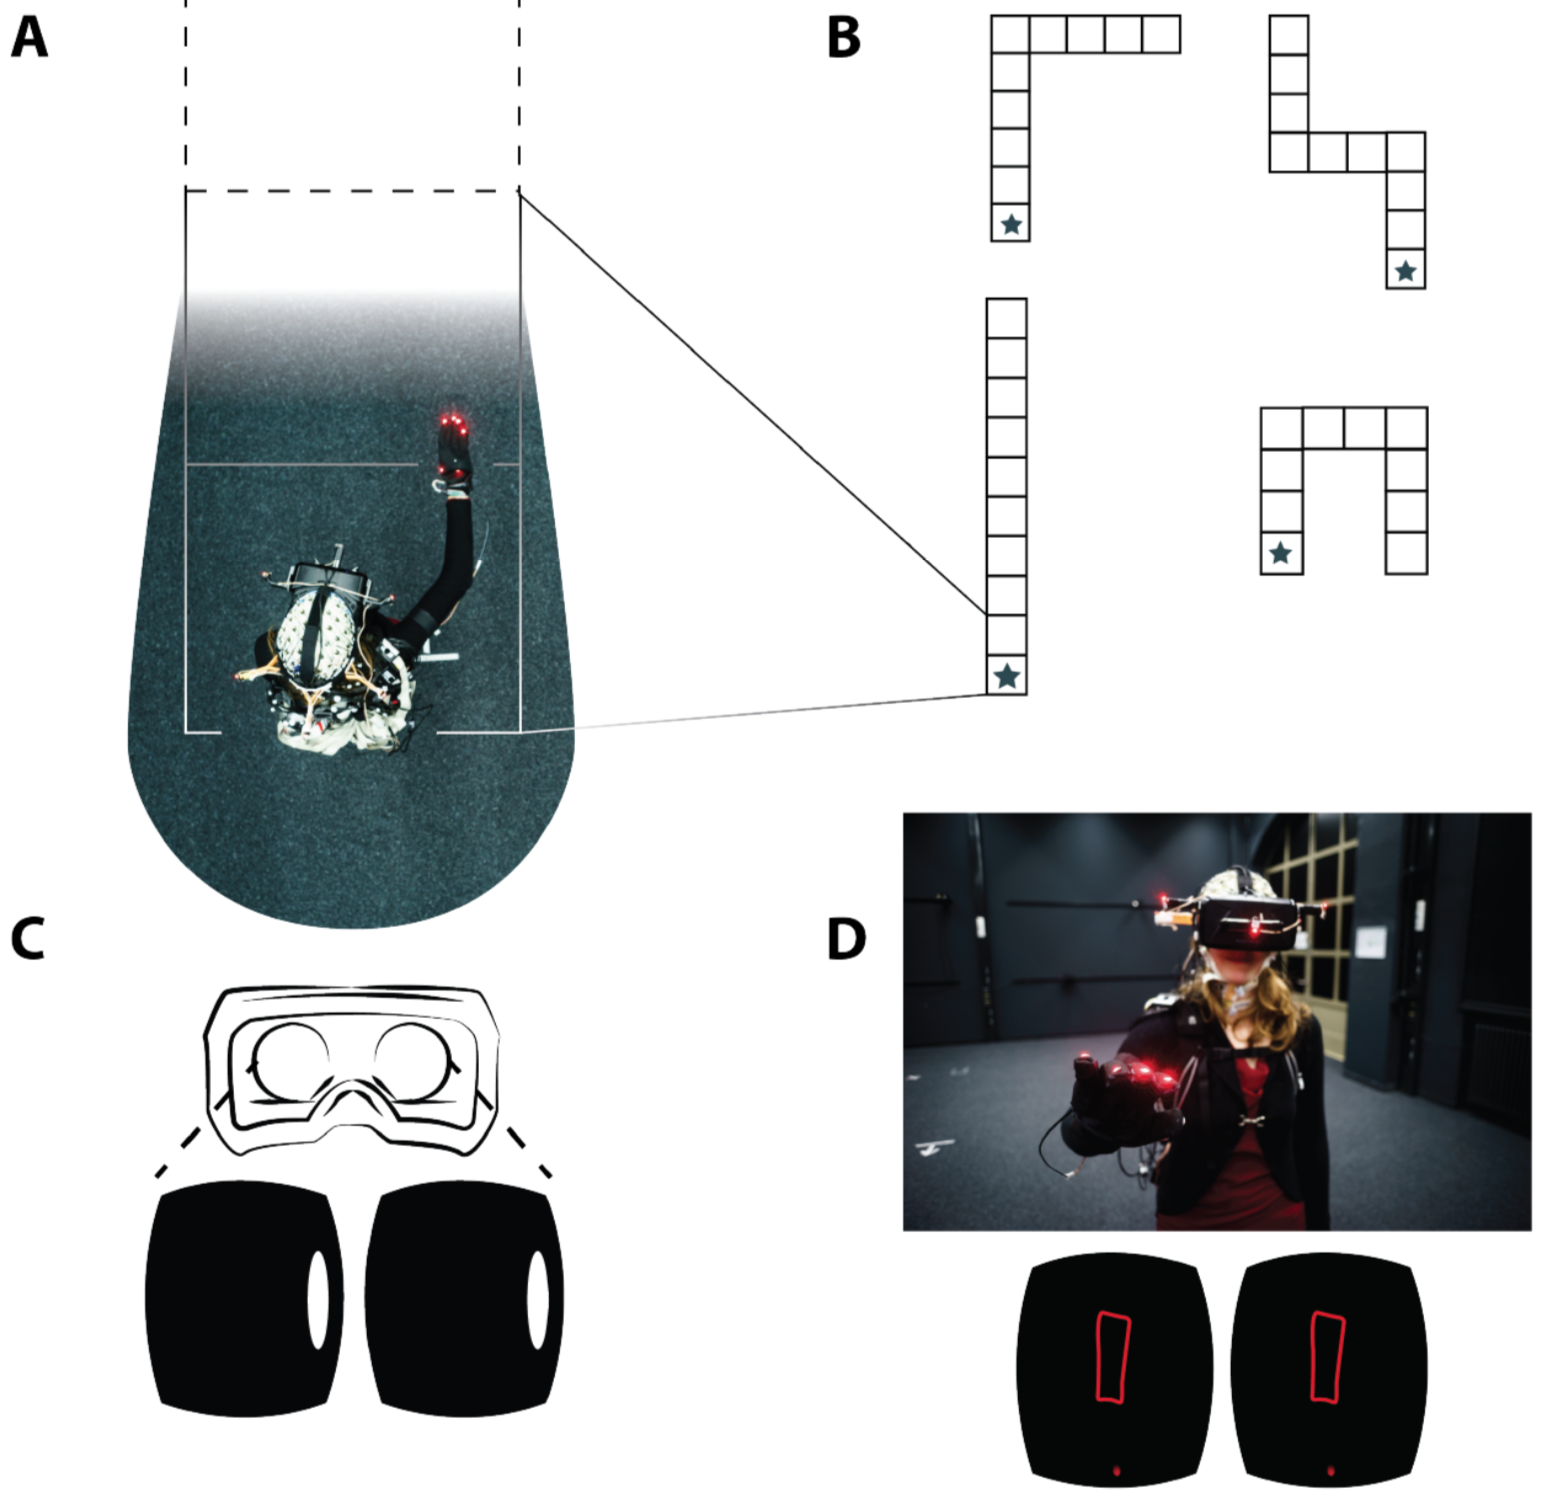
\includegraphics[width=\linewidth]{figures/IMT_Task.png}
    %\vspace{0pt}
    \caption{Invisible Maze Task, \textbf{A} Participant from a bird’s eye view. \textbf{B} Participants are instructed to explore four different mazes and return to the start. \textbf{C} First-person view in binocular `VR optics' of a wall touch. \textbf{D} Top: Participants draw a top-down view of the explored maze. Participant is equipped with 160 channels wireless EEG, head-mounted virtual reality goggles and LEDs for motion capture. Bottom: drawn sketch map. Find a detailed description in \cite{Gehrke2018}}
    \label{imt_task}
\end{figure}
Considering individual differences, our core analyses exhibits how differences in subjectively reported experienced presence impacts participants movement profiles. We follow up with a classification scheme predicting presence on an individual differences level. Video game experience, biological sex as well as spatial perspective taking skills proved to be significant predictors of a rich presence experience and were able to predict presence to within 3/4 of a point accuracy on a standard questionnaire scale. As a concurrent effect, we present an easily adaptable and scalable GLM analyses framework to investigate movement behavior with a high spatial resolution.